\documentclass[main]{subfiles}
\begin{document}

%@@@@@@@@@@@@@@@@@@@@@@@@@@@@@@
% Main Topics: extreme  rays, recession cones and representation of polyhedra 
% Representation of Polyhedra - 12.10.2017
% author: Vanessa Leite

\section{Representation of Polyhedra}
Definition: Let $\mathcal{P} = \{x \in \mathbb{R}^n \mid Ax \leq b\}$ be a 
polyhedron. $dim(\mathcal{P}) = n - dim(\{A_{i\cdot} \mid A_{i\cdot}x = b_i$, $
\forall x \in \mathcal{P} \})$ (implicitly linearly independent equations).

For $I \subseteq \{1, \dots, m\}$, $F = \{ x \in \mathcal{P} \mid A_{i\cdot} x = 
b$, $\forall i \in I \}$ is a face of $\mathcal{P}$.
Extreme case: $F = \emptyset$, $F = P$.\\

Vertices are faces of dimension $0$. Edges are faces of dimension $1$. Facets 
are faces of dimension $dim(\mathcal{P})-1$.\\

When $b = 0$, $\mathcal{P}$ is a cone. A cone is \textbf{pointed} if it does not 
contain a line.\\

For $\mathcal{P}$ and a point $y \in \mathcal{P}$, $\underbrace{rec}
_{\text{recession}}(y, \mathcal{P}) = \{ d \in \mathbb{R}^n \mid y + \lambda d 
\in \mathcal{P}$, $\forall \lambda \geq 0 \}$. If $\mathcal{P}$ is bounded then 
$rec(y, \mathcal{P}) = \{ 0 \}$, $\forall y \in \mathcal{P}$. \\

\paragraph{Observation:}
if $\mathcal{P} = \{x \in \mathbb{R}^n \mid Ax \leq b \}$, then the recession
cone $rec(y, \mathcal{P}) = \{d \in \mathbb{R}^n \mid Ad \leq 0 \}$, $\forall y
\in \mathcal{P}$. Therefore for every point $y \in \mathcal{P} \rightarrow
rec(y, \mathcal{P}) = rec(\mathcal{P}) = \{ d \in \mathbb{R}^n \}$.

\subparagraph{Proof of observation:}
Take $y \in \mathcal{P}$, $rec(y, \mathcal{P}) = \{d \in \mathbb{R}^n \mid y +
\lambda d \in \mathcal{P}$, $\forall \lambda \geq 0 \}$, now we claim this is
the same as $\{d \in \mathbb{R}^n \mid Ad \leq 0 \} = \mathcal{Q}$.\\

"$Q \subseteq rec(y, \mathcal{P})$": if $d \in \mathcal{Q} \rightarrow Ad \leq
0 \underbrace{\rightarrow}_{\forall y \in \mathcal{P}} A (y + \lambda d) = Ay +
\underbrace{\lambda}_{\geq 0} \underbrace{A d}_{\leq 0} \leq b$. \\

"$rec(y, \mathcal{P}) \subseteq Q$": Suppose it is not true, so, there exists
$i$, such that for $d \in rec(y, \mathcal{P}) \rightarrow A_{i\cdot}d > 0$. $y+ \lambda d
\in \mathcal{P}$, $\forall \lambda \geq 0 \rightarrow A_{i\cdot} (y + \lambda
d) = A_{i\cdot}y + \lambda A_{i\cdot} d \leq b_i \rightarrow \lambda \leq
\frac{b_i - A_{i\cdot}y}{A_{i\cdot}d}$, which contradicts $\lambda > 0$.


\emph{Remark: For a polyhedron in standard form $P=\{x \in \mathbb{R}^n_+ \mid
Ax = b \}$, $rec(\mathcal{P}) = \{d \in \mathbb{R}^n_+ \mid Ad = 0 \}$. }\\

From lecture 3, we know that if we take a matrix $A \in \mathbb{Z}^{m\times n}$
and a cone $C = \{x \in \mathbb{R}^n \mid Ax \leq 0 \}$. Then $(a) \iff (b)
\iff (c)$:
\begin{itemize}
\item (a) $0$ is an extreme point
\item (b) $C$ is pointed
\item (c) the dimension of all inequalities should be $n$ ($dim(\{A_{i\cdot} 
\mid i = 1, \cdots, m \}) = n$). 
\end{itemize}

A cone can not have more than one extreme point. In fact, for all $x \in C$ if
$x \neq 0 \rightarrow x = \frac{1}{2}[\frac{1}{2}x + \frac{3}{2}x]$ (there is
no linear combination to represent $x$ (?) - it seems that x can be written as
a linear combination).

\todo[inline]{check above information!}

\paragraph{Definition: Let the cone $C =\{x \in \mathbb{R}^n \mid Ax \leq 0\}$.
$x \in C$, $ x \neq 0$ is called an extreme ray of $C$ if the dimension of all
the tight constraints at this point is $n-1$ ($dim(\{A_{i\cdot} \mid i \in
I(x)) = n-1$}.\\
For $\mathcal{P} = \{x \in \mathbb{R}^n \mid Ax \leq b \}$ an extreme ray of
$\mathcal{P}$ is an extreme point of $rec(\mathcal{P})$.

\paragraph{Remark: Extreme rays of $C$ are faces of $C$ with dimenstion $1$. 
From now on, if $A \in Q^{m \times n}$, extreme rays are scaled to be integers 
whose $gcd = 1$.}

\begin{figure}[!h]
  \label{fig:cone}
  \centering
    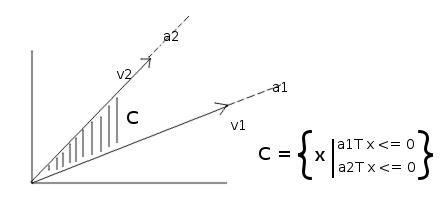
\includegraphics[width=0.5\textwidth]{imgs/cone.png}
\end{figure}

$C = \{x \mid x =\lambda_1 v_1 + \lambda_2 v_2, \lambda_1, \lambda_2 \geq 0 \}$
$v_1$ and $v_2$ are the extreme rays of $C$.\\
Can you give a point $c^T x \geq 0$? If $v_1$ and $v_2$ are $\geq 0$ then yes.
Otherwise, we have a point that is false.

\paragraph{Theorem: Take a polyhedron $P = \{x \in \mathbb{R}^n \mid Ax \leq b
\}$ with at least one extreme point.} What happens if $\displaystyle \max_{x
\in \mathcal{P}} c^{T} x = +\infty$? This can happen iff there is an extreme
ray $d \in \mathcal{P}$, such that $c^T d > 0$.

\subparagraph{Proof:}
Suppose $d$ extreme ray of $\mathcal{P}$, $c^T d > 0$. $P \neq \emptyset$. Take
a point $x \in \mathcal{P}$. By definition of extreme rays, $Ad \leq 0$, hence
$x + \lambda d \in \mathcal{P}$, $\forall \lambda \geq 0$.\\
$\rightarrow c^T(x +\lambda d) = c^T x + \lambda c^T d \xrightarrow[\lambda \to
\infty]{} +\infty$.

Conversely, $\displaystyle \max_{x \in \mathcal{P}} c^{T} x = +\infty$, shows 
that exists an extreme ray. Write down a dual problem.
\todo[inline]{homework}

Consider that the dual $\min b^T y$, $st. A^T y = c$, $y \geq 0$ has no
solution. We know that $\min 0^T y$, $st. A^T y = c$, $y \geq 0$ is infeasible.
Consider now the cone problem: $\max c^T x$, $st. Ax \leq 0$. This problem is
either unbounded or infeasible. $0$ is feasible for our problem, so,
$\max c^T x$, $st. Ax \leq 0$ is unbounded. As $\max c^T x$ is unbounded,
$\max c^T x = +\infty$.\\

$\mathcal{P}$ has at least one extreme point, therefore has no lines, and in
particular, $dim(\{A_{i\cdot} \mid i = 1, \dots, m\}) = n$. If $\mathcal{P}$
does not have a line, then the cone does not have a line, i.e,
$rec(\mathcal{P})$ is pointed.
Under this assumption in the cone, prove that exists a recession ray in the
cone such that $c^T d > 0$.
\todo[inline]{homework: Start by taking any point of the polyhedron (check 
lecture 03)}

\paragraph{Theorem: Let $\mathcal{P} = \{x \in \mathbb{R}^n \mid Ax \leq b\}$
with at least one extreme point. Let $\{v^1, \dots, v^k\}$ be all the extreme
points in $\mathcal{P}$ and $\{w^1, \dots, w^r\}$ be all the extreme rays in
$\mathcal{P}$. \\ Then $\mathcal{P} = \mathcal{Q} = \{ \sum_{i =1}^{k}
\lambda_i v^i + \sum_{j=1}^{r} \mu_j w^j \mid \lambda \geq 0$, $\mu \geq 0$,
$\mathtt{1}^T \lambda =1 \}$}
In other words: every point of a bounded polyhedron can be writed as a convex
combination of the vertices and extreme rays of the polyhedron.

\subparagraph{Proof:} "$\mathcal{Q} \subseteq \mathcal{P}$" and "$\mathcal{P} \subseteq \mathcal{Q}$"\\

"$\mathcal{Q} \subseteq \mathcal{P}$"\\
Take an arbitrary point $x \in \mathcal{Q}$. $x = \sum_{i =1}^{k} \lambda_i v^i
+ \sum_{j=1}^{r} \mu_j w^j$, $\lambda \geq 0$, $\mu \geq 0$. We know $A w^j
\leq 0$, $\forall j$, $Av^i \leq b$, $\forall i$.
$\mathcal{P}$ convex $\rightarrow \sum_{i=1}^{k} \lambda_i v^i = y \in
\mathcal{P}$, $\lambda_i \geq 0$, $\mathtt{1}^T \lambda = 1$.
$\rightarrow z = \sum_{j = 1}^{r} \mu_j w^j$ satisfies $Az \leq 0$. $x = y + z$
satisfies $Ax = \underbrace{Ay}_{\leq b} + \underbrace{Az}_{\leq 0} \leq b
\rightarrow x \in \mathcal{P}$.

"$\mathcal{P} \subseteq \mathcal{Q}$"\\
Assume the statement is not true. This implies there exists $z \in \mathcal{P}$
and $z \notin \mathcal{Q}$.
Then, $R = \max \sum_{i = 1}^{k} 0\lambda_i + \sum_{j=1}^{r} 0 \mu_j$, $st.
\sum_{i = 1}^{k} \lambda_i v^i + \sum_{j = 1}^{r} \mu_j w^j = z$, $\lambda_i$,
$\mu_j \geq 0$, $\mathtt{1}^T \lambda = 1$. If $z \notin \mathcal{Q}$, $R$ is
infeasible, so the dual problem is unbounded. The dual of $R$ is
$\max p^T z + q$, $st. p^T v^i + q \leq 0$, $p^T w^j \leq 0$, $\forall i =1,
\dots, k$, $\forall j = 1, \dots, r$.

Which means $p = 0$ and $q = 0$ is feasible $\rightarrow R$ is unbounded.
$\rightarrow \exists (p^*, q^*)$ such that $(p^*)^T z + q^* > 0 \geq (p^*)^T
v^i + q^*, \forall i = 1, \dots, k$, $(p^*)^T w^j \leq 0$, $\forall j = 1,
\dots, r$. \\

$\rightarrow (p^*)^T w^j \leq 0$, $\forall j = 1, \dots, r$, $(p^*)^T v^i <
(p^*)^T z$, $\forall i = 1, \dots, k$.(*)

Consider $\displaystyle \max (p^*)^T x$, $st. Ax \leq b$, which is feasible ($
\mathcal{P} \neq \emptyset$).

Suppose, $\displaystyle \max_{x \in \mathcal{P}} (p^*)^T x = +\infty$, then we 
know from previous theorem that exists an extreme ray $j$ such that $(p^*)^T 
w^j > 0$, but this contradicts (*).

Suppose, $\displaystyle \max_{x \in \mathcal{P}} (p^*)^T x$ is finite, i.e,
there exists an extreme point $v^i$ , $i \in \{1, \dots, k\}$ attaining the
optimal solution. Since $z \in \mathcal{P}$, then $(p^*)^T v^i \geq (p^*)^T z$,
which contradicts (*).

So, this contradicts that $\exists z \in \mathcal{P}$, $z \notin \mathcal{Q}$.

\subsection{Remarks}

\paragraph{A pointed polyhedron can be written as the convex hull of its
vertices plus the convex hull of its extreme rays ($\mathcal{P} = conv(V) +
cone(E)$), where $V$ are the vertices and $E$ the extreme rays of $\mathcal{P}
$}.

What if $\mathcal{P}$ does contain a line? e.g. $\{x \in \mathbb{R}^2 \mid x_2
\geq 1 \} =
\underbrace{\begin{pmatrix} 0 \\ 1 \end{pmatrix} + cone (\begin{Bmatrix} 0 \\ 1
\end{Bmatrix})}_{\text{pointed}} + cone(\underbrace{\{ \begin{pmatrix} 1 \\ 0
\end{pmatrix}, \begin{pmatrix} 1 \\ 0 \end{pmatrix} \}}_{\in ker(A)})$

This idea can be generalized: Let $\mathcal{P} = \{x \in \mathbb{R}^n \mid Ax
\leq b \}$ for $A \in \mathbb{Q}^{m \times n}$, $b \in \mathbb{Q}^m$ be a
polyhedron containing a line.

Let $d = dim(ker(A))$, $L \in \mathbb{Q}^{n \times d}$ be a matrix whose column
vectors form a basis of $ker(A)$, and $Q \in \mathbb{Q}^{n \times n-d}$ be a
matrix st. its columns form a basis for $Im(A^T)$. Recall from linear algebra
that if we get the two basis together we form a basis for the entire space.
$[L | Q]$ forms a basis of $\mathbb{R}^n$ and that $\forall \mu \in \mathbb{R}
^{n-d}\setminus \{0\}$. $AQ\mu \neq 0$.\\

$\mathcal{P} = \{L \lambda + Q \mu \mid \lambda \in \mathbb{R}^d$, $\mu \in
\mathbb{R}^{n-d}$, $Ay \leq b\}$ = this is a Mikowski's sum = $\{L \lambda \mid
\lambda \in \mathbb{R}^d \} + \underbrace{ \{ y \in \mathbb{R}^n \mid y = Q\mu, 
\mu \in \mathbb{R}^{n-d}, Ay \leq b \} }_{= \mathcal{P}'}$.

$\mathcal{P}'$ does not contain a line. Let $d \in \mathbb{R}^n$ st $d= Q
\alpha$, $\alpha \in \mathbb{R}^{n-d}$, and $Ad =0$, then, $d=0$, so, indeed,
$\mathcal{P}$ does not contain a line.

\paragraph{Corollary of representation theorem:} Let $\mathcal{P}$ be a
polyhedron, $\mathcal{P} = \{x\in \mathbb{R}^n \mid Ax \leq b \}$. Then, exist
finite sets $V$ and $E$ such that $P = conv(V) + cone(E) + lin(L) = conv(V) +
cone(E, L, -L)$. $lin(L) = \{x \in \mathbb{R}^n \mid x = L \lambda$, $\lambda
\in \mathbb{R}^d \}$.


\subsection{Supplementary Reading - Section 4.8 and 4.9 from [BT97]}
\todo[inline]{update}

\end{document}